\subsection{Auckland}

Comencemos por describir la ruta generada:
Se han realizado 22 saltos hasta alcanzar el destino solicitado, de los cuales en el $72 \% $ de los mismos aproximadamente, hemos obtenido respuestas del tipo $TIME\_EXCEEDED$, determinando así que el largo de nuestra ruta es de 16 saltos, y que del resto de los valores del $TTL$ no hemos obtenido respuesta alguna. Como también se puede ver en la figura \ref{mapa-auckland}, y en el cuadro \ref{tabla-auckland}, durante el trayecto se realizaron 3 saltos intercontinentales. Por otra parte, el método de Cimbala nos ha detectado en un principio todo número positivo como outlier, pero al sacar los 0s sólo ha detectado aquellos que se muestran en el cuadro ya mencionado.

\begin{table}[!htbp]
\centering
\caption{My caption}
\label{tabla-auckland}
\begin{tabular}{|c|c|c|c|}
\hline
\textbf{TTL} & \textbf{IP}    & \textbf{COUNTRY} & \textbf{OUTLIERS} \\ \hline
1   & 10.0.2.2        & Undefined     &               \\ \hline
6   & 200.89.161.133  & Argentina     & {[}outlier{]} \\ \hline
7   & 200.89.165.5    & Argentina     &               \\ \hline
8   & 200.89.165.250  & Argentina     &               \\ \hline
9   & 190.216.88.33   & Argentina     &               \\ \hline
10  & 67.17.94.249    & Australia     & {[}outlier{]} \\ \hline
13  & 4.68.127.54     & United States &               \\ \hline
14  & 129.250.4.250   & United States &               \\ \hline
15  & 129.250.2.219   & United States & {[}outlier{]} \\ \hline
16  & 129.250.7.69    & United States & {[}outlier{]} \\ \hline
17  & 129.250.3.123   & United States &               \\ \hline
18  & 204.1.253.166   & United States &               \\ \hline
19  & 202.158.194.172 & Australia     & {[}outlier{]} \\ \hline
20  & 182.255.119.139 & Australia     &               \\ \hline
21  & 210.7.39.251    & New Zealand   &               \\ \hline
22  & 210.7.39.178    & New Zealand   & {[}outlier{]} \\ \hline
\end{tabular}
\end{table}

\newpage

\begin{figure}[!htbp]
  \centering
    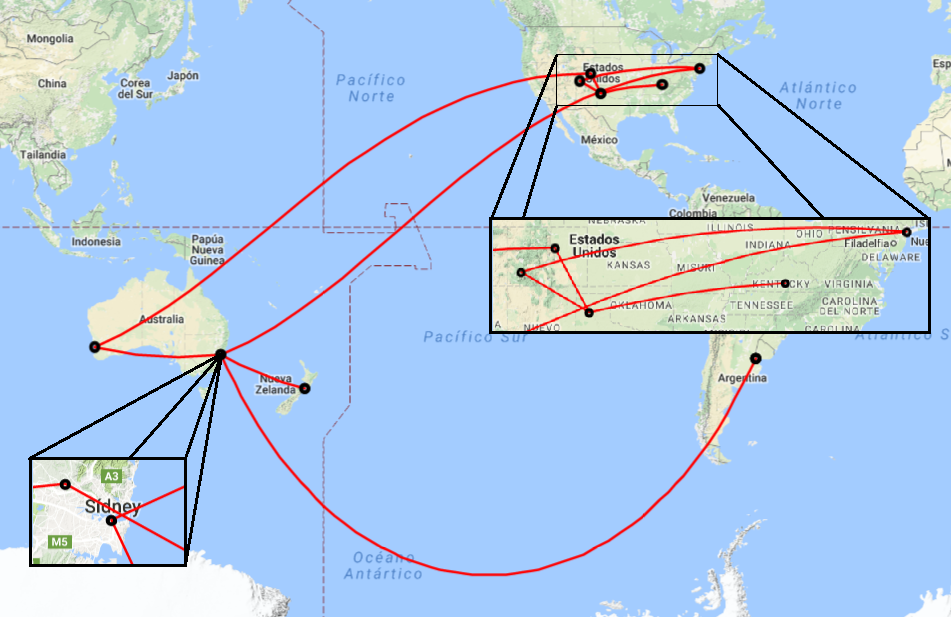
\includegraphics[scale=0.6]{imagenes/auckland-graficos/mapa-auckland.png}
  \caption{auckland- RTT hops}
  \label{mapa-auckland}
\end{figure}

ACÁ IRÍA EL CHAMUYO DE AUCKLAND

\begin{figure}[!htbp]
  \centering
    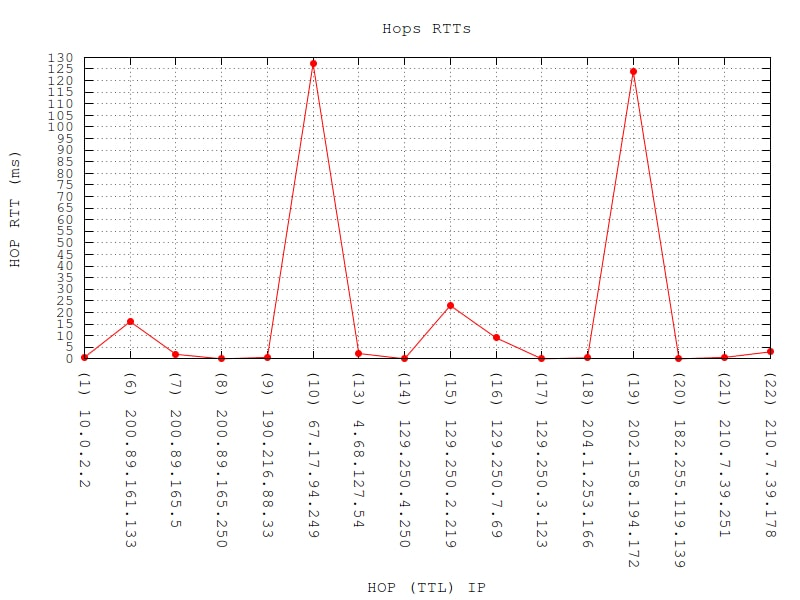
\includegraphics[scale=0.6]{imagenes/auckland-graficos/traceroute-auckland.jpg}
  \caption{auckland- RTT hops}
  \label{fig:7}
\end{figure}

En la figura \ref{fig:7} se puede observar como el ttl 10 y 19 tienen un rtt claramente distinguido del resto.

\begin{figure}[!htbp]
  \centering
    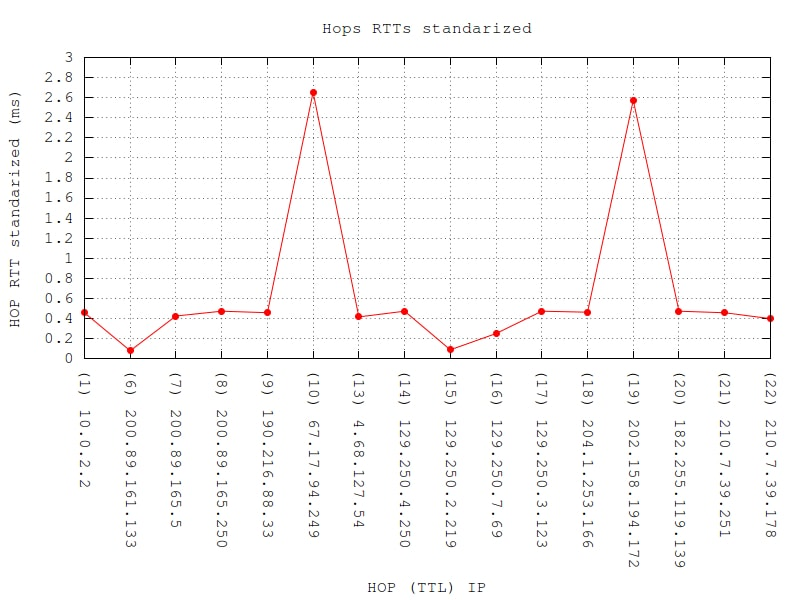
\includegraphics[scale=0.6]{imagenes/auckland-graficos/traceroute-auckland-standarized.jpg}
  \caption{auckland- RTT hops standarized}
  \label{fig:8}
\end{figure}

En la figura \ref{fig:8} se puede observar una situacion similar a la de la figura \ref{fig:7}.


